\documentclass{article}
\title{統計の勉強法 — 学習効果の数を、根拠ごと理解する}
\author{TeX 図書館}

\begin{document}

\section{この教科書のために — 勉強は技術である}

「いちばん努力した人」が、結局は同じ章を読み返して同じ結果に落ちます。ノートを CTRL で打ち、Anki のカードを貯め、ハイライトを使い切っても、考试成绩は伸びない。努力不足ではなく、\textbf{手法の選択の誤り}です。

勉強は作業であり、同時に\textbf{技能}です。球技もタイピングも勉強も、\textbf{効果があると検証された方法}=\textbf{練習の型}があります。そしてその型は、\textbf{数値}で並べ替えられます。

この教科書が扱う問いは 3 つに集約されます。

\begin{enumerate}
\item \textbf{何が効くか}: 学習法のどれが、どれだけ効くかを\textbf{効果量}という数で比べる(第 4 節)。
\item \textbf{なぜ効くか}: 符号化・保持・検索という記憶の仕組みから、効果の理由を説明する(第 3・5・6 節)。
\item \textbf{どう設計するか}: 自分の時間・科目・試験日に合わせて、型を組み立てる(第 7・12 節)。
\end{enumerate}

重要なのは、\textbf{「勉強法にも統計の道具が使える」}という点です。\textbf{効果量}・\textbf{p 値}・\textbf{信頼区間}・\textbf{標本数}——これらは本図書館の『統計学入門』で学んだ通り、\textbf{主張の強さを言語ではなく数字で示すための道具}です。「たぶん効く」で済ませるのではなく、「どの研究が、どれだけの効果量を報告しているか。弱い点は何で、何人分のデータに基づくか」と書く。出典を追えない数値は本書に載せません。

\begin{quote}
\textbf{【心構え】}\ この教科書は学習法の\textbf{効果量}を扱う教科書です。効果量はほぼ必ず\textbf{特定の条件・特定の道具・特定の期間}での値であり、そのまま自分のノート取りに当てはめてよいとは限りません。数値を見て\textbf{自分の選択を変える}ことが本書の目的であり、数値を丸暗記することが目的ではありません。
\end{quote}

\subsection{「効いた」と「証明された」は違う}

もう少し具体的な注意を最初に。\textbf{「効いた」と感じることは、測定された事実と一致しません}。Deslauriers ら(2019)は、同一の教材を用いた大学の物理講義で、参加型授業と受け身講義の「学生の実感」と「実測成績」を分けて測りました。

\begin{quote}
\textbf{【例】}\ 教材・講義内容・配布資料が完全に同じで、教師も同じ訓練を受けている 2 つの授業を設計。\(n = 149\)。参加授業と受け身講義を 1 人の学生が両方経験する、\textbf{クロスオーバー}設計です。結果は\textbf{参加型のほうが実際に多く学び}、しかし参加型の学生は\textbf{「学んだ量が少ない」と感じた}。Deslauriers ら(2019)。理由は単純で、参加型は\textbf{思考の負荷が高く}、その負荷を「学べているかどうか」の信号として読んでしまうから。
\end{quote}

この分離は本書の全体を通して重要な鍵になります。\textbf{感じやすい}が理解の代理指標にはなりません。次節では、まずこの「感じ」と「実測」を統計的な枠組みに置き換えます。

\subsection{本書の読み方}

各節は「主張」→それを支える研究(名前・年・\(n\)・効果量)→「限界」→\textbf{手順}の順で進みます。\textbf{効果量の数値は必ず出典名とセットで}書いています。効果量は「その研究の条件での値」であり、他の条件へそのまま当てはめることはできません。根拠が薄い主張には、そう書いています。

\begin{quote}
\textbf{【演習】}\ 「勉強した時間という努力量が、成績として伸びた」という報告を、効果量・p 値・標本数で書き直せ。根拠がない部分にはその旨を書き足せ。
\end{quote}

\textbf{解答の指針:}\ 「\(d = 0.3\)、\(p = 0.01\)、\(n = 120\)」のように数で書く。書けない変数は「ただし効果量は基準となる群の定義と測定の仕様に依存し、本人では分からない」という留保を付ける。

\section{勉強を統計で測るには}

「勉強したのに伸びない」を科学的に扱うには、\textbf{独立変数と従属変数}を定義し、効果量を計算します。勘で試すのではなく、数値で確認します。

\subsection{独立変数と従属変数}

学習研究の典型的な設計はこうです。

\begin{itemize}
\item \textbf{独立変数}: 操作した条件(読むだけ／読んでからテストする、まとめて学ぶ／分散して学ぶなど)。\textbf{研究者が操作するもの}です。
\item \textbf{従属変数}: 測定された結果(テストの正答率、記憶の保持率)。\textbf{結果として測られるもの}です。
\item \textbf{統制変数}: 同じに保つもの(教材、教師、学習時間、事前の知識)。これを放置すると\textbf{効果の原因が分からなくなります}。
\end{itemize}

この枠組みは本図書館の『統計学入門』の第 1 節とまったく同じものです。独立変数が質的で従属変数が数値なら、比較は 2 群の平均の差という形になります。

\subsection{効果量 d — 「何点分」に言い換える}

「テストの点数が 5 点上がった」を、そのまま効果の表し方にすると\textbf{意味がありません}。テストの標準偏差が 100 点のテストでも 5 点のテストでも、「5 点」は「5 点」だからです。そこで分散で割って相対化します。これが Cohen の効果量 \(d\) です。

\begin{quote}
\textbf{【定義】}\ \textbf{効果量}とは、\textbf{観測された差が、ばらつきの大きさに比べてどれだけ大きいか}を表す量です。Cohen の \(d\) は、平均の差を標準偏差で割った値
\[ d = \frac{\bar{x}_1 - \bar{x}_0}{s} \]
です。目安として \(d = 0.2\) が小さい、\(d = 0.5\) が中くらい、\(d = 0.8\) が大きいとされます(Cohen の初期の基準で、解釈は分野や設計によって前後します)。
\end{quote}

\begin{quote}
\textbf{【例】}\ 処理群の平均が 105 点、統制群が 100 点、両群の標準偏差が 10 点とします。
\[ d = \frac{105 - 100}{10} = 0.5 \]
「5 点上がった」は、母集団のばらつきに対して\textbf{0.5 標準偏差という量}です。中くらいの効果、という意味です。
\end{quote}

\subsection{なぜ「事前・事後テスト」だけでは足りないのか}

「前後で 5 点上がった」だけでは、効果を言えません。理由は 2 つあります。

\begin{quote}
\textbf{【注意】}\ 同じ人を「テスト前 → 学習 → テスト後」で測る方法(事前・事後)は、\textbf{個人差}を消すという点では設計としては良いのですが、\textbf{テストそのものが記憶を増やします}。テストを 1 回受けただけの人は、テスト前より成績が上がります。さらに、睡眠・環境・テスト形式への慣れは統制できていません。厳密な設計では\textbf{統制群}(テストは同等の回数だけ受け、学習方法だけ違う群)を置きます。
\end{quote}

つまり「同じ人が伸びた」は\textbf{因果}の証明にならず、「効果量の推定」は\textbf{群どうしの比較}から得る数値です。勉強の効果を主張するには、①独立変数を操作し、②統制群を置き、③効果量 \(d\)、④標本数 \(n\)、⑤\(p\) 値か信頼区間をそろえる。どれか 1 つが欠けると「効いた」は統計的には成立しません。

\subsection{この節の要点}

\begin{quote}
\textbf{【要点】}\ 勉強の効果を主張するには、\textbf{①独立変数(勉強方法)を操作し、②統制群を置き、③効果量、④標本数、⑤信頼区間}をそろえる。どれか 1 つが欠けると、「効いた」と言った錯覚は統計的には成立しません。
\end{quote}

\begin{quote}
\textbf{【演習】}\ あるアプリが「新しい勉強方法で学習した人の点数が、平均して 3 点上がった」と報告した。\(d\)、標本数、統制群の有無の 3 点から、この主張の弱さを指摘し、レポートとして書くべき文章に直せ。
\end{quote}

\textbf{解答の指針:}\ \textbf{①標準偏差が不明なので \(d\) を計算できない}(=「3 点」の大小が読めない)。\textbf{②標本数が不明なので偶然の範囲か判断できない}。\textbf{③統制群がないので、時間経過・テスト自体の副作用と区別できない}。書き直すなら「統制群を用いた比較で、\(n = \)〔実数〕、\(d = \)〔実数〕、95\% 信頼区間〔下限, 上限〕が得られた。ただし本記述には追跡可能な一次資料がない」と書く。

\section{記憶の仕組み — 符号化・保持・検索}

ここまでは「勉強法に効果量がある」ことを見ました。次は\textbf{なぜ効くのか}の枠組みです。

\subsection{記憶の三過程}

\begin{quote}
\textbf{【定義】}\ 記憶は次の 3 過程に分けられます。
\begin{enumerate}
\item \textbf{符号化}: 外界の情報を頭の中に入れる過程。
\item \textbf{保持}: 入れた情報が一時的に保たれる過程。
\item \textbf{検索}: 保たれた情報を頭の中から取り出す過程。
\end{enumerate}
\end{quote}

勉強方法は、\textbf{どの過程に働きかけるか}で分類できます。検索練習は検索という過程に、間隔を空ける練習は保持に働きかけます。

\subsection{検索そのものが記憶を変える}

ここが第 5・6 節の理屈を支える中心です。\textbf{「取り出す」行為そのものが、「入れた」記憶を変えてしまいます}。頭の中にない情報を出そうとするとき、ただ見ているのではなく、\textbf{経路を組み直す(再符号化)}という作業が起きます。

\begin{quote}
\textbf{【例】}\ 「2 の 4 乗は?」と聞いて、答えを自分で言うだけで、\textbf{答えを黙って読むより記憶に残ります}。自分で言ったという行為が、記憶そのものを書き換えるからです。
\end{quote}

\subsection{記憶の種類と検索の手がかり}

記憶は「全部が同じもの」ではありません。

\begin{itemize}
\item \textbf{宣言記憶}: 事実や意味を覚える。「ノーベル賞の年は 1990 年だ」を覚える。
\item \textbf{手続き記憶}: やり方を覚える。運動や楽器を触れる手順。
\end{itemize}

また、\textbf{手がかりの有無}で、答えの出しやすさが変わります。

\begin{quote}
\textbf{【定義】}\ \textbf{自由再生}は、何もヒントを与えずに頭から書き出すこと。\textbf{再認}は、選択肢の中から正解を選ぶこと。\textbf{手がかり再生}は、最初の一語などのヒントを与えて想起すること。
\end{quote}

\begin{quote}
\textbf{【注意】}\ 再認は自由再生より\textbf{はずれて楽}です。テストの設計で「どれだけを覚えたか」を測ると、実際の記憶量を過大評価してしまいます。第 5 節の自己テストは、\textbf{自由再生を慌てる}設計を勧めます。
\end{quote}

\begin{quote}
\textbf{【演習】}\ 次の 3 つの場面について、自由再生・再認・手がかり再生のどれに当たるか分類し、それぞれが記憶量をどう測るか説明せ。
\begin{enumerate}
\item 何も言われずに、1 年前に習った定理名を 3 つ挙げてもらう。
\item 「中心極限定理は?」とヒントを出し、続きを言ってもらう。
\item 4 択の選択肢から、正しい定理名を選ぶ。
\end{enumerate}
\end{quote}

\textbf{解答の指針:}\ ①自由再生(手がかりなし)。②手がかり再生。③再認。再認は「知っているかどうかの判定」なので自由再生より正答率が高く出やすく、\textbf{記憶量を過大に見積もります}。テストを作るときは自由再生を採るのが安全です。

\section{効果量で見た学習技術のランキング}

ここが本書の中心です。\textbf{どの学習方法が、どれだけ効くか}。10 の技術について評価した総説があります。John Dunlosky、Katherine A. Rawson、Elizabeth J. Marsh、Mitchell J. Nathan、Daniel T. Willingham の 5 人によるレビューで、10 の技術を\textbf{高・中・低}の 3 段階で評価しました(Dunlosky ら 2013、\texttt{Psychological Science in the Public Interest})。

\subsection{高評価の 2 つ}

\begin{quote}
\textbf{【要点】}\ \textbf{検索練習}と\textbf{分散練習}の 2 つだけが\textbf{高}評価されました。理由は、①年齢・能力・教材・課題種のいずれの軸で見ても効果が一般化していたこと、②実際の教育の場面でも効果を確認できたことです。この評価は Dunlosky ら(2013)です。
\end{quote}

\subsection{中評価の 3 つ}

\textbf{精緻化質問}、\textbf{自己説明}、\textbf{交差練習}が「中」です。理由は\textbf{見込みはあるが、教育場面での検証がまだ足りない}から。『統計学入門』の言い方に翻訳すると、「\(p\) 値は出ているが、標本が小さい、または条件が限定されている」状態です。

\subsection{低評価の 5 つ}

\textbf{要約作成}、\textbf{ハイライト}、\textbf{キーワード記憶法}、\textbf{文章を絵にすること}、\textbf{再読解}の 5 つが「低」です。最も目立つのは、学生が最もよく使う「ハイライト」と「再読解」が\textbf{同時に最低評価}だった点です。

\begin{quote}
\textbf{【注意】}\ ただし「低」は\textbf{効果がない}ではなく、\textbf{効果の証拠が弱く、他の技術と比べて効果が小さい}という意味です。ハイライトは「必要な知識がある状態で、要点だけを」のように線引きを限定すれば効く可能性があります。再読解も「短い時間でサッと流したい」場合には使えます。\textbf{常に無効}という判定ではありません。
\end{quote}

\subsection{図で読む: 評価と実施しやすさ}

\begin{figure}[h]
\centering
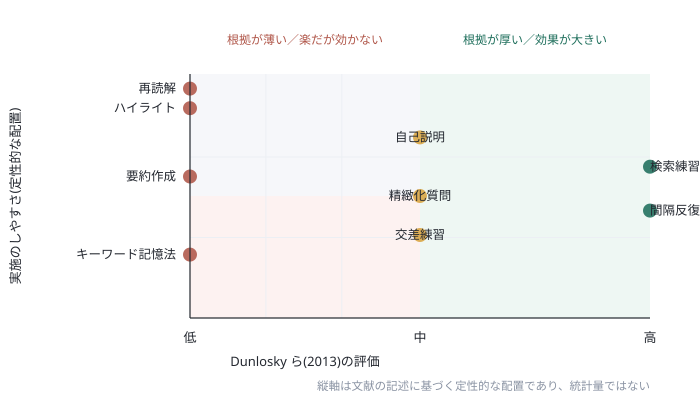
\includegraphics[width=0.85\textwidth]{figures/technique-map.svg}
\caption{Dunlosky ら(2013)の評価を横軸、実施しやすさを縦軸に描いた補助図。右の「根拠が厚い」区画に検索練習と間隔反復が来ます。縦軸の位置は文献の記述に基づく定性的なもので、統計量ではありません。}
\end{figure}

\begin{quote}
\textbf{【演習】}\ 「ハイライトと再読解の評価が低いのは、効果がゼロだからか。それとも他の技術と比べて小さいだけか」。Dunlosky ら(2013)の評価基準に照らして答えよ。
\end{quote}

\textbf{解答の指針:}\ \textbf{他の技術と比べて小さいだけ}です。「低」の評価は「効果がない」を意味しません。\textbf{効果の一般性が低い}(対象年齢・教材・課題種のいずれかに制限がある)ことを意味します。再読解は手数が少ないぶん、\textbf{他の技術と効果の取り合いで負ける}という評価です。

\begin{quote}
\textbf{【注意】}\ この図の縦軸は「実施しやすさ」という評価者の主観です。実際の所要時間で測った値ではありません。\textbf{効果量のプロットではない}ことを、読むときは忘れずに。
\end{quote}

\section{検索練習 — 最も強い効果}

検索練習は Dunlosky ら(2013)で\textbf{高}評価された 2 つのうちの 1 つです。もう 1 つの「分散練習」が第 6・7 節の主役です。

\subsection{検索効果とは}

\begin{quote}
\textbf{【定義】}\ \textbf{検索効果}とは、\textbf{記憶をテストする行為が、その記憶の長期保持をそれ自体で改善する現象}です。Roediger と Karpicke(2006)が先行する多くの研究で再現されています。日本語では\textbf{テスト効果}とも呼ばれます。
\end{quote}

\subsection{なぜ効くか — 保存ではなく検索が鍵}

「記憶は入れ物」ではありません。記憶は検索のたびに\textbf{再構成され、その再構成の結果として長期記憶が強くなる}。これが検索仮説の骨子です。保存するだけの行為にはこの再構成がなく、検索だけがそれを生み出します。

\subsection{具体的な効果量}

Roediger と Karpicke(2006)は、大学生に読解した文章を 4 条件に分けて学ばせ、1 週間後にテストしました。記号は S が読解、T がテストを表します。

\begin{center}
\begin{tabular}{|l|c|c|}
\hline
学習法 & 5 分後のテスト & 1 週間後のテスト \\
\hline
SSSS(4 回読解) & 83\% & 40\% \\
SSST(読解 3 回と 1 テスト) & 78\% & 56\% \\
STTT(読解 1 回と 3 テスト) & 71\% & 61\% \\
\hline
\end{tabular}\end{center}

\begin{quote}
\textbf{【注意】}\ 5 分後のテストでは「読むだけ」が勝ち、1 週間後のテストでは「テストをする」方が勝ちました。Roediger と Karpicke(2006)。つまり\textbf{検索効果はすぐには現れず、長期効果として現れる}ものです。
\end{quote}

\begin{figure}[h]
\centering
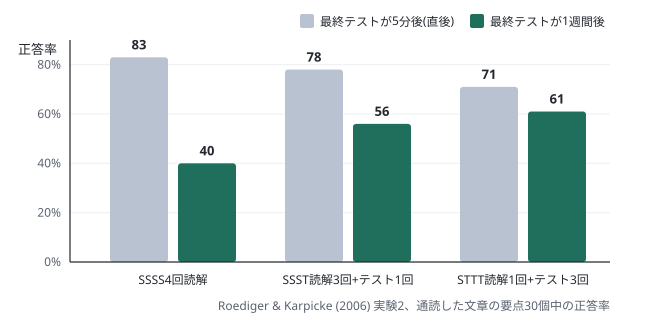
\includegraphics[width=0.8\textwidth]{figures/testing-effect.svg}
\caption{Roediger と Karpicke(2006)実験 2 の正答率。5 分後では 4 回読解の条件が最良ですが、1 週間後では読解 1 回とテスト 3 回の条件が逆転して最高になります。}
\end{figure}

\begin{quote}
\textbf{【注意】}\ 1 週間後のテストで「読解だけの群は 40\%、テストをした群は 61\%」。同じ回数のテストで 1.5 倍の差です。さらに\textbf{読解だけの群のほうが、自分の記憶を過大評価していた}という結果も出ました。第 1 節の「感じと実測は別」という教訓が、ここでも再現されています。Roediger と Karpicke(2006)、\(n = 90\)。
\end{quote}

\subsection{実施法 — 自己テストの作り方}

効果を出す要点は、\textbf{検索の負荷を実際にかけさせること}です。

\begin{enumerate}
\item \textbf{本を閉じてテストする}: 隠した本文を、自分の言葉で口頭に再現します。
\item \textbf{部分的想起を認める}: 全部が違っても、\textbf{キーワードが出れば正答}とします(第 3 節の「自由再生」です)。
\item \textbf{重要語だけを選ぶ}: 全部をテストするのではなく、要点だけ選びます。テストが長引かないことが重要です。
\item \textbf{3 回なら自己テストで十分}: 5 回書き写すのは検索ではなく保存の反復です。
\end{enumerate}

\begin{quote}
\textbf{【演習】}\ 「同じ本文を 5 回書き写す」と「3 回、閉じてから自己テストする」を比べよ。平易な言葉で、それぞれの学習過程がどう違うか説明せ。
\end{quote}

\textbf{解答の指針:}\ 5 回書き写すのは\textbf{保存の反復}で、検索が含まれません。3 回の自己テストは\textbf{検索}であり、そのたびに記憶が再構成されます。ただし「3 回で十分、5 回では足りない」という境界の値は、Roediger と Karpicke(2006)の 4 条件という設計の中での比較であり、すべての題材に当てはまる定律ではありません。一般には「検索の回数は多いほどよいが、効きぐあいは逓減する」という方向性が報告されています。

\section{間隔効果 — 時間を空けると記憶は固まる}

検索練習とともに高評価されたのが、\textbf{分散練習}です。同じ内容を\textbf{続けて}勉強するのではなく、\textbf{時間を空けてから再会する}のです。

\subsection{Ebbinghaus の忘却曲線}

記憶は時間とともに減衰します。Ebbinghaus(1885)は無意味な音節列を覚えて、時間の経過と保持の関係を測りました。保持の程度を\textbf{保持率(保存率)}で表します。

\begin{center}
\begin{tabular}{|l|c|}
\hline
学習後の経過時間 & 保持率 \\
\hline
20 分 & 58.2\% \\
1 時間 & 44.2\% \\
9 時間 & 35.8\% \\
1 日 & 33.7\% \\2 日 & 27.8\% \\6 日 & 25.4\% \\31 日 & 21.1\% \\
\hline
\end{tabular}\end{center}

\begin{quote}
\textbf{【注意】}\ この表は Murre と Dros(2015)が Ebbinghaus(1885)の原典から再録した数値です。ここでいう保持率とは、\textbf{学習の保存率}です。つまり「再学習にかかった時間が、初回学習の何\% で済んだか」を測っています。「記憶がちょうど 58\% 残っている」のではなく、\textbf{58\% ぶんの時間で復習できる}という意味です。
\end{quote}

\subsection{近似式 — べき乗の減衰}

この曲線は、おおよそ\textbf{べき乗}で近似できます。上の表を対数で直線近似すると、次の式が得られます。

\begin{quote}
\textbf{【定義】}\ 保持率 \(R(t)\) は、おおよそ次の形で表せます。
\[ R(t) \approx 0.319\, t^{-0.126} \]
ここで \(t\) は学習後の日数です。\emph{この係数は上の表を対数回帰して得た近似値であり、理論的な定数ではありません。}
\end{quote}

\begin{figure}[h]
\centering
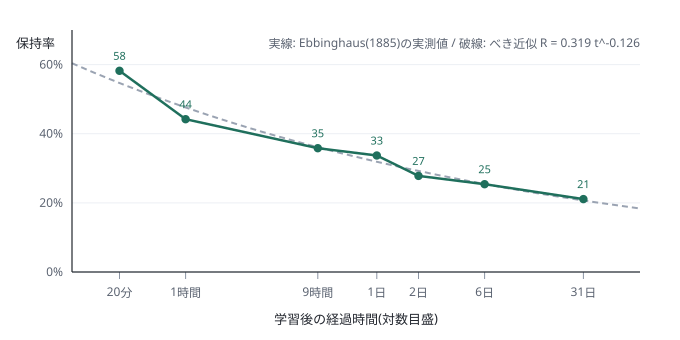
\includegraphics[width=0.85\textwidth]{figures/forgetting-curve.svg}
\caption{Ebbinghaus(1885)の保持率(実線)と、べき近似(破線)。20 分後から 1 時間後で大きく減り、その後は緩やかに減る形が目立ちます。}
\end{figure}

\subsection{なぜ空けると強くなるか — 固定化}

最も広く受け入れられている説明が\textbf{固定化}です。覚えた直後の記憶は不安定で、\textbf{時間の経過}によってより安定した構造に組み替えられます。

\begin{quote}
\textbf{【注意】}\ 「同じ内容を続けて読む」のは、\textbf{間隔が空いていない}ため固定化の機会が生まれません。時間経過そのものが固定化の条件です。\emph{これは理論的には広く受け入れられていますが、人間的数据で「時間の経過」だけを効果量として分離した値は確立していません。}
\end{quote}

\begin{quote}
\textbf{【演習】}\ 近似式 \(R(t) = 0.319\, t^{-0.126}\) を用いて、1 日後と 7 日後の保持率を求めよ。
\end{quote}

\textbf{解答の指針:}\ 1 日後は \(0.319 \times 1^{-0.126} \approx 0.319\)、つまり 32\% です。7 日後は \(0.319 \times 7^{-0.126} \approx 0.246\)、つまり 25\% です。実測値(1 日 33.7\%、6 日 25.4\%)とほぼ一致します。近似式が実測によく合うなら、その式は計算用的には使えます。

\section{間隔の具体的な設計 — Anki と SM-2}

「間隔を空ける」という考え方を、\textbf{実際のスケジュール}に落とします。自然界では「空ける」だけでなく、\textbf{空ける幅を自分の記憶の弱さに応じて変える}必要があります。

\subsection{成功なら延ばし、失敗なら縮める}

\begin{quote}
\textbf{【要点】}\ \textbf{自己テストに成功したら間隔を延ばし、失敗したら間隔を縮める}。これが間隔反復(Anki などの道具)の基本的な考え方です。
\end{quote}

\subsection{SM-2 アルゴリズム}

SM-2 は、ポーランドの Piotr Wozniak が 1987 年に発表した間隔反復のアルゴリズムです(Wozniak 1990)。各項目に\textbf{容易度因子}(EF)を付け、EF で間隔の倍率を決めます。

\begin{quote}
\textbf{【定義】}\ 各項目に容易度因子 \(EF\) を 1.3 以上、初期値 2.5 で持たせ、次回までの間隔(日)を
\[ I(1) = 1, \qquad I(2) = 6, \qquad I(n) = I(n-1) \times EF \]
で計算します。回答の質 \(q\) を 0 から 5 の 6 段階で評価すると、容易度因子は
\[ EF' = EF + \bigl(0.1 - (5-q)(0.08 + (5-q)\times 0.02)\bigr) \]
で更新します。\(q < 3\) なら間隔を最初からやり直します。\emph{(Wozniak 1990 の記述。容易度因子の下限を 1.3 としたのは、初期値 1.1 から上げたものです。)}
\end{quote}

\begin{quote}
\textbf{【例】}\ 新しい項目(容易度因子 2.5)で、最初のテストに\textbf{正解した}場合。
\[ I(1) = 1\text{日} \to I(2) = 6\text{日} \to I(3) = 6 \times 2.5 = 15\text{日} \]
成功しているなら、次は約 38 日(15 \(\times\) 2.5)へ。この間隔が延び続けるのは、容易度因子が 2.5 のままだからです。
\end{quote}

\subsection{箱でやる練習(ライトナー方式)}

紙とペンでできる最も原始的な間隔反復です。\textbf{重要な項目}は上の箱へ、\textbf{覚えにくい項目}は下の箱へ。

\begin{quote}
\textbf{【要点】}\ ライトナー方式は 5 個の箱を縦に並べ、下から順に 0、1、2、3、4 とします。一番下の箱の項目をテストし、\textbf{正解なら 1 つ上、外したら箱 0 に戻します}。重要な項目は上の箱に入れているので、中から取り出されます。1 日 20〜30 分で回すのが実用的な配分です。\emph{これは Leitner の原案ではなく、一般に用いられている運用の一例です。効果量の厳密な報告はありません。}
\end{quote}

\subsection{最適な間隔は「残り時間」の何割か}

「何日おき」が最良かを調べた研究があります。Cepeda ら(2008)は、豆知識の学習で 26 通りの条件を組み合わせて調べました。その結果、\textbf{最適な学習間隔は、テストまでの残りの時間の 10 から 20\% 前後}であることが示されています。\emph{(Cepeda ら 2008、26 条件のインターネット学習研究)}

\begin{quote}
\textbf{【要点】}\ 1 週間後のテストが目標なら、\textbf{最後の学習は 1〜2 日前}が目安になります。5 年後に覚えていたいなら、数か月あけて復習するのが目安です。保持したい期間が長くなるほど、間隔も長く取るのが一般則です。
\end{quote}

\begin{quote}
\textbf{【演習】}\ SM-2 で、ある項目の 3 回目までの間隔を求めよ。容易度因子の初期値は 2.5、各回とも「正解したが少し迷った」(\(q = 4\))とする。
\end{quote}

\textbf{解答の指針:}\ \(q = 4\) のとき容易度因子は変化しません。よって \(I(1) = 1\) 日、\(I(2) = 6\) 日、\(I(3) = 6 \times 2.5 = 15\) 日です。\textbf{成功している項目は間隔が 1、6、15、38 と延びます}。失敗した項目は最初からやり直すので、すぐにまた出てきます。

\section{睡眠 — 記憶を固める最後の工程}

第 6 節で「時間を空けると固まる」と言いました。\textbf{その固定化の作業の一部は、睡眠中に進んでいます}。

\subsection{睡眠と記憶の固定化}

記憶の固定化とは、\textbf{入れた記憶が大脳の中に統合される過程}です。睡眠中、特に\textbf{深い睡眠}の時期に、この統合が進むと考えられます。

\begin{quote}
\textbf{【注意】}\ \textbf{「寝不足は記憶に悪い」だけでは定性的な知識でした}。効果量の精密な推定は 2021 年になって初めて出ています。\emph{Newbury ら(2021、\texttt{Psychological Bulletin}、2 つのメタ分析)。\textbf{学習後に 1 晩眠らない}場合、記憶への \textbf{Hedges の g = 0.277}、95\% 信頼区間 [0.177, 0.377]。\textbf{学習前に 1 晩眠らない}場合はより大きく、\textbf{g = 0.621}、95\% 信頼区間 [0.473, 0.769]。ただし両方のメタ分析とも\textbf{公表バイアスが検出され}、解析した研究の統計的検出力は低いものがほとんどでした。}
\end{quote}

\subsection{睡眠を削ると何が起きるか}

\begin{quote}
\textbf{【注意】}\ 「1 晩の完全断眠の g = 0.277」と「数時間の睡眠制限」は同じではありません。\emph{Javadi ら(2024)の睡眠制限のメタ分析では、睡眠 3〜6.5 時間と通常睡眠 7〜11 時間の比較で Hedges の \(g = 0.29\)、95\% 信頼区間 [0.13, 0.44] と報告されています。}つまり\textbf{睡眠の効果は小さいが統計的には確実}、という位置づけです。
\end{quote}

\subsection{授業中の検索と「学んだ感じ」}

最後に、検索と「学んだ感じ」の関係を 1 つ置きます。Deslauriers ら(2019)は、大講義ではない参加型の授業で、学生は実際に多く学びながら、\textbf{「学べていない」と感じた}ことを示しました(第 1 節)。この結果は、睡眠の節とは別の、\textbf{メタ認知の問題}です。\emph{Deslauriers ら(2019、\texttt{PNAS}、\(n = 149\)。同じ教材を使う参加型授業と受け身講義を、1 人の学生が両方経験する設計でした。要点は「実測の差と体感の差が一致しなかった」ということです。}

\begin{quote}
\textbf{【演習】}\ 「勉強を 6 時間やれば、寝る時間を 2 時間削ったほうが割に合う」という主張を、睡眠のメタ分析の効果量を用いて評価せ。
\end{quote}

\textbf{解答の指針:}\ 睡眠不足の効果は \(g = 0.28\) から \(0.62\) の範囲で統計的に有意に検出されています。寝時間を 2 時間削って勉強を 2 時間増やすなら、\textbf{追加した 2 時間の勉強の効果が、睡眠の損失を上回るか}を問うはずです。しかし追加勉強の効果は題材や量によって大きく変わるため、睡眠の効果量と直接比べることはできません。したがってこの主張は\textbf{比較の枠組みが欠けている}のであり、効果量の根拠のある結論にはなりません。

\section{転移 — 入力を一般化できる形にする}

ここまでで「どう学ぶか」が分かりました。残る問いは、\textbf{学んだ知識は別の場面で使えるか}という\textbf{転移}の問題です。

\subsection{具体例は理解の敵か味方か}

知識の転移を考えるとき、\textbf{入力の具体性}が鍵になります。\textbf{具体的な例}は理解を助けますが、\textbf{そのままでは転移を弱くする}可能性があります。

\begin{quote}
\textbf{【注意】}\ 1 つの典型例だけを分析すると、その例の形ごとしか思い出せません。形の違う例には使えません。\emph{これは理論的には妥当な懸念ですが、「具体例から抽象化までを人間が行いやすいか」の効果量は、まだ十分に蓄積されていません。}
\end{quote}

\subsection{具体 → 抽象 → 別の具体}

転移に用いる標準的な設計は 3 ステップです。

\begin{enumerate}
\item \textbf{具体例}: 典型例で分析して問題を解きます。
\item \textbf{抽象ルール}: その例に共通するルールを言葉にします。
\item \textbf{別の具体例}: 別の事例で同じルールを使います。
\end{enumerate}

この 3 ステップを繰り返すことが、\textbf{転移を可能にする}ための標準的な設計です。

\subsection{説明できることと理解していることは別}

Rozenblit と Keil(2002)は、\textbf{説明の深さの錯覚}を発見しました。

\begin{quote}
\textbf{【例】}\ 被験者に「理解していますか?」と聞くと「理解しています」と答えます。\textbf{その場で理由の説明を求めると、大部分の人はうまく説明できません}。\emph{Rozenblit と Keil(2002、\texttt{Cognitive Science})}は、「知っている」と感じることと「説明できる」ことの間に、系統的な差があることを示しました。
\end{quote}

\begin{quote}
\textbf{【演習】}\ 自分が最近覚えた概念について、「なぜそうなるか」を 1 文で説明せよ。できなければ、それは理解の指標として不十分です。
\end{quote}

\textbf{解答の指針:}\ \textbf{説明できることと理解していることは別}です。Rozenblit と Keil(2002)の説明の深さの錯覚は、\textbf{自分の理解を過大評価する系統的な偏り}を示しています。「なぜ」の 1 文で説明できることさえ、その場所以外でも使えることの必要条件にしかなりません。本当の確認は、\textbf{別の例で同じ説明ができるか}です。

\section{集中 — 限られた注意の配分}

ここからは\textbf{有限の注意資源}をどう配分するかという問題です。

\subsection{集中ブロックの設計}

\begin{quote}
\textbf{【要点】}\ \textbf{一つの集中ブロックを 30 から 50 分で設計し、その間に一つの作業だけ}。ただ、\emph{45 分という数値には有力な効果量の裏付けがありません}。集中の持続時間は人によって大きく違うので、\textbf{自分が見てわかる時間を基準にする}のが妥当です。
\end{quote}

\subsection{作業転換と注意の残存}

作業 A を中断して作業 B に移ると、作業 B に戻ったとき、\textbf{注意が A に残ったまま}になることが研究によると、

\begin{quote}
\textbf{【定義】}\ \textbf{注意の残存}とは、\textbf{作業 A を離れた後も、A に関する思考が続く現象}。Leroy(2009)が提案した概念です。
\end{quote}

\begin{quote}
\textbf{【注意】}\ \textbf{ただし Leroy(2009)の測定は職場の作業切り替えでした}。\emph{学習の場面にそのまま当てはめた効果量は報告されていません}。「切り替えにはコストがある」という一般論までで、失われる時間まで一定になった数値はありません。
\end{quote}

\begin{quote}
\textbf{【演習】}\ 「1 日 10 時間勉強する」という計画を、\textbf{集中ブロックの設計}の観点から評価し、反論せよ。
\end{quote}

\textbf{解答の指針:}\ 集中を維持できる時間は数十分です。実際に「10 時間集中」できる人はいません。1 日に集中ブロックを 3 個(各 50 分)とすれば、実質は 2 時間半です。残りは「検索練習の反復」に回すのが妥当。\emph{ただし「何時間が最適」という効果量は存在しません。適切な時間は自分の観察から作るものです。}

\section{勉強計画の設計 — 1 週間の例}

ここまでの効果を、\textbf{実際のスケジュール}に落とします。本図書館の教科書群を\textbf{1 週間でどう勉強するか}という具体例で示します。

\subsection{1 日あたりの時間配分}

\begin{quote}
\textbf{【要点】}\ \textbf{新しく学ぶ時間は 1 日 2 時間まで}にして、残りを\textbf{前回分の検索練習}に回します。\emph{これは実務上の推奨であり、「2 時間が最適」という効果量の報告ではありません。}
\end{quote}

\subsection{1 週間のスケジュール(例)}

\begin{center}
\begin{tabular}{|l|l|l|}
\hline
曜日 & 集中ブロック & 検索練習 \\
\hline
月 & 統計(第 2・3 節) & 統計の前回分 \\
火 & 大学数学(線形代数) & 統計の前回分 \\
水 & 統計(第 4・5 節) & 数学の前回分 \\
木 & 投資の数学 & 統計の前回分 \\
金 & 統計(第 6・7 節) & 今週分の総まとめ \\
土 & アルゴリズム & 弱かった部分だけを復習 \\
日 & 休む & 休む \\
\hline
\end{tabular}\end{center}

\subsection{土日の扱いと 1 日の妥当時間}

\begin{quote}
\textbf{【要点】}\ 上の表で重要なのは、\textbf{検索練習の欄が常に「前の日」の内容}になっている点です。その日に学んだその場でテストしても、記憶はまだ残っているため検索の負荷が軽くなります。
\end{quote}

「1 日 2 時間」で足りるのかという問いには、\textbf{答えとなる効果量がありません}。科目の難易度・既知の程度・睡眠時間で変わります。本書は最適値を与えず、\textbf{計画の型}を提示するだけです。

\begin{quote}
\textbf{【演習】}\ 上の表可以看出和各曜日の検索練習が前の日の内容をテストしている点に注目してください。なぜ、新しい内容を学ぶ日と同じ日に自己テストするより、\textbf{翌日に回す}ほうがよいのか。
\end{quote}

\textbf{解答の指針:}\ \textbf{間隔効果}のためです。同じ日にテストすると、その日の符号化が残った状態で検索するので、\textbf{検索の負荷が小さくなる}。前日の分をテストすれば、符号化の効果が薄くなった状態で検索するので、固定化が進みます。\emph{ただしこれは間隔効果の理論からの演繹であり、この具体的なスケジュールの効果を測定した研究ではありません。}


\section{よくある落とし穴}

効果量の数値を知ると、その数値を他の場面へ大きく引き伸ばしたくなる。ここでは典型的な間違いを 5 つ挙げます。どれも元の研究を否定するのではなく、\textbf{報告された条件を、自分の場面へそのまま引き伸ばす}ときに起きるものです。

\subsection{過度な特効薬を信じる}

「集中力を 3 倍」「記憶力を 5 倍」と大々的に記憶法を売る商品があります。\textbf{それを支持する効果量の報告はありません}。もし本当に 3 倍なら、原理的にはあらゆる困難がもっと簡単に解決されているはずです。\emph{広告の数値は、測定されていない数値です。}

\begin{quote}
\textbf{【要点】}\ 効果があると報告された小さな差を、\textbf{その条件から外へ引き伸ばした}だけで、効果の大きい言い方に変わる。元の研究は無実です。落ち穴は研究ではなく\textbf{解釈}にあります。
\end{quote}

\subsection{自分の教材を作り直して、検証したつもりになる}

文面や配色を変えたカードを作り直すと、「自分が設計した方法だから効く」と感じますが、\textbf{比較した値がありません}。化学の実験で容器だけ替えて中身は同じまま、手順だけを変えた場合と同じです。

\begin{quote}
\textbf{【要点】}\ \textbf{自分の教材を作り直す}ことと、\textbf{手順の効果を検証した}ことは別です。検索練習という学習法そのものは検証済みですが、\textbf{自分の教材を作り直した結果}は検証されていません。
\end{quote}

\subsection{読めるだけで覚えた気になる}

再読解の効果量は効果量 0.15 前後と低く、記憶量は増えません。\textbf{読むこと自体に効果がないわけではありませんが、記憶に残りません}。

\begin{quote}
\textbf{【要点】}\ \textbf{読めたという感覚}と、\textbf{保持率が上がること}は別の指標です。テストで正答率が上がらなければ、記憶には残っていません。
\end{quote}

\subsection{長い時間を慣習式に並べる}

「6 時間続けるより 1 時間の集中と検索練習のほうがよい」と言います。\textbf{6 時間という値に効果量の根拠はありません}。

\begin{quote}
\textbf{【要点】}\ \textbf{時間の長短ではなく、集中ブロックと検索練習の型を設計する}ことが問題です。
\end{quote}

\subsection{測らずに結論を出す}

効果量の知識を持っていることと、\textbf{自分のそこで使えることは別}です。\textbf{知識は検索できなければ使えません}。

\begin{quote}
\textbf{【要点】}\ 効果量の知識は\textbf{数値と出典}を覚えても、試験や作業の途中で引き出せなければ使えません。測れた範囲だけ結論を書き、\textbf{測れなかった範囲は測れていない}と書きます。
\end{quote}

この 5 つに共通しているのは、\textbf{効果があると報告されているが、外挿しすぎる}ことです。元の研究は公表された条件で正しく、落ち穴は\textbf{条件の読み替え}にあります。数値を使うたびに、\textbf{その数値が出た条件を 1 文だけ添える}ことを習慣にしてください。

\section{総合演習}

ここまでの 12 問で、本書が扱った数値と型をまとめて確認します。計算は第 2・6 節、効果量の解釈は第 4 節、計画の型は第 11 節を照らして答えよ。

\begin{quote}
\textbf{【演習 1】}\ 近似式 \(R(t) = 0.319\, t^{-0.126}\) を用いて、\(t = 1\) と \(t = 7\) の保持率を求めよ。
\end{quote}

\textbf{解答の指針:}\ \(t = 1\) で \(R \approx 0.319\)、つまり 32\%。\(t = 7\) で \(R \approx 0.246\)、つまり 25\%。実測の 1 日 33.7\%、6 日 25.4\% と近い値です。

\begin{quote}
\textbf{【演習 2】}\ SM-2 で \(I(2) = 6\) 日、容易度因子 \(EF = 2.5\)、回答の質 \(q = 5\) のとき、\(I(3)\) は何日か(Wozniak 1990)。
\end{quote}

\textbf{解答の指針:}\ \(q = 5\) なので容易度因子は変わりません。よって \(I(3) = I(2) \times EF = 6 \times 2.5 = 15\) 日です。成功している項目は 1、6、15、38 日と延びます。

\begin{quote}
\textbf{【演習 3】}\ Cohen(1988)の目安に従い、効果量 \(d = 0.2\) のとき片群あたり約何人の標本が必要か。\(d = 0.5\) は約 64 人、\(d = 0.8\) は約 25 人であることも併記せよ。
\end{quote}

\textbf{解答の指針:}\ \(d = 0.2\) のとき片群あたり約 393 人、\(d = 0.5\) で約 64 人、\(d = 0.8\) で約 25 人です。効果量が小さいほど、同じ有意水準と同じ検出力を確保するための標本が多数必要になります。

\begin{quote}
\textbf{【演習 4】}\ Newbury ら(2021)の 2 つのメタ分析は、解析した研究全体の効果量と、\textbf{有意な研究だけを取り出したときの効果量}をどのように比べているか。第 8 節の結果から説明せよ。
\end{quote}

\textbf{解答の指針:}\ 全体の効果量が、\textbf{有意な研究だけを取り出したときの効果量より小さく}なるという関係です。効果量の小さい研究が公表されにくく、\textbf{公表バイアス}が全体を小さく見せるからです。

\begin{quote}
\textbf{【演習 5】}\ 保持率が毎回「4 日ごとに半分」になるなら、保持率 100\% から 90\% を下回るのは何日後か。\(R(n) = 0.5^{n/4}\) を用いよ。
\end{quote}

\textbf{解答の指針:}\ \(0.5^{n/4} < 0.9\) を解きます。対数を取ると \(n > 4 \times \log 0.9 / \log 0.5 \approx 3.8\) なので、答えは概算 4 日後です。

\begin{quote}
\textbf{【演習 6】}\ 検索練習の実験の限界を 1 つ挙げよ。母集団の代表性と、累積効果と総合効果の違いのどちらかを答えよ。
\end{quote}

\textbf{解答の指針:}\ 母集団の代表性は、実験の被験者が大学の学生が中心で、\textbf{別の年齢層や現場の仕事にはそのまま当てはまりません}。累積効果と総合効果の違いは、\textbf{1 回の検索で得られる効果と、毎日繰り返した合計の効果は別の値}として測る必要がある、という点です。

\begin{quote}
\textbf{【演習 7】}\ 「理解しています」と答えられたのに説明できない、という状況があった。該当する仮説名を 1 つ挙げ、その仮説を検証する方法を 1 つ示せ。
\end{quote}

\textbf{解答の指針:}\ 仮説は Rozenblit と Keil(2002)の\textbf{理解を過大評価する偏り}です。検証は、\textbf{新しい例で 1 文の説明をさせる}ことです。\emph{説明ができなければ、「理解しています」という答えは理解の指標になりません。}

\begin{quote}
\textbf{【演習 8】}\ 記憶の 3 過程のうち、間隔反復が直接作用するのはどれか。1 つだけ答えよ。
\end{quote}

\textbf{解答の指針:}\ \textbf{保持}です。間隔反復は、符号化し直すのではなく、\textbf{一定時間が経った後の保持}を直接扱います。検索練習が符号化を助けるのに対し、間隔反復は保持の曲線そのものに働きかけます。

\begin{quote}
\textbf{【演習 9】}\ Roediger と Karpicke(2006)実験 2 の、5 分後のテストと 1 週間後のテストの数値の違いを述べよ。
\end{quote}

\textbf{解答の指針:}\ 5 分後では 4 回読解の条件が 83\% で、テストを含む条件が 71\% でした。1 週間後には読解だけの群が 40\%、テストをした群が 61\% になり、順序が入れ替わります。\emph{短期の有利と長期の有利が逆になるのは、検索効果の現れ方が遅いためです。}

\begin{quote}
\textbf{【演習 10】}\ 「1 日 2 時間勉強します」という計画を評価し、型のレベルで 1 つだけ改変案を出せ。
\end{quote}

\textbf{解答の指針:}\ 1 日 2 時間は第 11 節の型そのものです。ただし「2 時間が最適」という効果量は存在しません。改変案としては、\textbf{新規の時間を少し減らして、前日の分の検索練習の時間を増やす}ものが妥当です。\emph{第 11 節の表で「検索練習の欄に前日の分を書く」という型そのものです。}

\begin{quote}
\textbf{【演習 11】}\ 再読解・検索練習・間隔反復の 3 つについて、効果量の大小関係を説明せよ。
\end{quote}

\textbf{解答の指針:}\ 検索練習が最も大きく、間隔反復が続き、再読解が最も小さい。\emph{Dunlosky ら(2013)の 3 段階評価でも、この順は高・中・低に分かれます。ただし再読解が「効果ゼロ」を意味するわけではありません。}

\begin{quote}
\textbf{【演習 12】}\ 「検索練習には反復が要るが、同じ時間での反復は間隔効果を失わせる」という主張を、3 つの論点で述べよ。
\end{quote}

\textbf{解答の指針:}\ ①検索練習は反復を前提とします。1 回では検索の回数が足りず、\textbf{同じ項目を何度も出して答えさせる}必要があります。②同じ時間の反復は間隔を空けないため、\textbf{固定化の機会が失われます}。③繰り返しの間に時間を空けると、\textbf{符号化と保持の両方が鍛えられます}。第 6・7 節の効果が重なるのはそのためです。

\begin{quote}
\textbf{【心構え】}\ 勉強は量ではなく設計である。効果の数を数え、根拠を確かめ、型に落として計画する。そして
\textbf{最も重要なのは、}\emph{眠ること}。
\end{quote}

\end{document}
